% VUT FIT MITAI
% MSZ 2021/2022
% Author: Vladimir Dusek
% Login: xdusek27

%%%%%%%%%%%%%%%%%%%%%%%%%%%%%%%%%%%%%%%%%%%%%%%%%%%%%%%%%%%%%%%%%%%%%%%%%%%%%%%%

\chapter{Asymetrická kryptografie, vlastnosti, způsoby použití, poskytované bezpečnostní funkce, elektronický podpis a jeho vlastnosti, hybridní kryptografie, algoritmus RSA, generování klíčů, šifrování, dešifrování.}

% Todo:
% - Matematicke problemy by sly formulovat lepe a formalneji. To co tu mam, by lehce nemuselo stacit. Kouknout k materialum od Mateje Kastaka.
% Kongruence, multiplikativni inverze

%%%%%%%%%%%%%%%%%%%%%%%%%%%%%%%%%%%%%%%%%%%%%%%%%%%%%%%%%%%%%%%%%%%%%%%%%%%%%%%%

\section{Metadata}

\begin{compactitem}
    \item Předmět: Kryptografie (KRY)
    \item Přednáška:
    \begin{compactitem}
        \item 6) Asymetrická kryptografie, vlastnosti, způsoby použití, poskytované bezpečnostní funkce.
        \item 7) Elektronický podpis a jeho vlastnosti, hybridní kryptografie.
        \item 8) Příklady asymetrických algoritmů, RSA.
    \end{compactitem}
    \item Záznam:
    \begin{compactitem}
        \item 2021-03-08
        \item 2021-03-22
    \end{compactitem}
\end{compactitem}

%%%%%%%%%%%%%%%%%%%%%%%%%%%%%%%%%%%%%%%%%%%%%%%%%%%%%%%%%%%%%%%%%%%%%%%%%%%%%%%%

\section{Úvod a kontext}

\textit{Viz. \uv{Úvod a kontext} v~předchozích otázkách z~tohoto předmětu.}

\paragraph*{Asymetrická kryptografie} \begin{compactitem}
    \item V~asymetrické kryptografii se používají páry klíčů (soukromý a veřejný). Soukromý je používán k~dešifrování, resp. vytvoření digitálního podpisu. Veřejný je používán k~šifrování, resp. ověření digitálního podpisu.
    \item Každý uživatel generuje svůj pár klíčů. Veřejný klíč je zveřejněn (znají ho všichni), sourkomý je držen v~tajnosti (zná ho pouze vlastník).
    \item Všechny asymetrické algoritmy jsou blokové.
    \item Asymetrické algoritmy jsou pomalejší než symetrické.
\end{compactitem}

\paragraph*{Způsoby použití} Asymetrická kryptografie lze využít k: \begin{compactitem}
    \item šifrování,
    \item digitálnímu podepisování,
    \item pro výměnu symetrického klíče (\textit{key exchange}).
\end{compactitem}

\paragraph*{Vlastnosti} Vlastnosti symetrické a asymetrické kryptografie\footnote{Otazníky -- částečně, za předpokladů, \dots}.
\begin{table}[H]
\begin{tabular}{lllll}
& Důvěrnost & Autentizace & Integrita & Nepopiratelnost \\
Symetrická & ano & ? & ? & ne \\
Asymetrická - šifrování & ano & ? & ? & ne \\
Asymetrická - podepisování & ne & ano & ano & ano \\
Asymetrická - kombinace & ano & ano & ano & ano
\end{tabular}
\end{table}

\bigskip\noindent\begin{minipage}{\linewidth}
\begin{lstlisting}[language=Python, caption={Kombinace klíčů obou stran u~asymetrický kryptografie. Pořadí operací může být i opačné.}]
# Odesilatel (A):
msg = encrypt(msg, SK_A) # necht msg je zprava k~odeslani
msg = encrypt(msg, PK_B)
send(msg_2)

# Prijemce (B):
msg = receive()
msg = decrypt(msg, SK_B)
msg = decrypt(msg, PK_A)
\end{lstlisting}
\end{minipage}

\paragraph*{Digitální podpis} Vytvoření digitálního podpisu konkrétních dat pomocí soukromého klíče podepisatele. Každý kdo zná veřejný klíč podepisatele, může pravost podpisu ověřit. Digitální podpis zajišťuje autentizaci, itegritu a nepopiratelnost.

\paragraph*{Algoritmy} Algoritmy asymetrické kryptografie se nedají \textit{vymyslet}, musí se objevit. Jsou založeny na těžkých matematických problémech. \begin{compactitem}
    \item Problém batohu (\textit{knapsack problem}) -- MH (Merkle-Hellman)
    \item Faktorizace čísel -- RSA (Rivest-Shamir-Adleman)
    \item Diskrétní logaritmus -- DSA (Digital Signature Algorithm), DH (Diffie-Hellman)
    \item Eliptické křivky -- ECDSA, ECDH
\end{compactitem}

\paragraph*{Problém batohu} Problém batohu je NP-úplný problém kombinatorické optimalizace. Nechť ${x_1, x_2, \dots, x_n}$ je množina objektů, každý objekt má svoji cenu $v_i$ a svoji hmotnost $w_i$, dále mějme batoh, který má kapacitu $W$. Cílem je vybrat takovou množinu objektů, jejichž hmotnost je menší nebo rovna $W$ a má nejvyšší možnou cenu\footnote{Problém má více obdobných variant.}. Formálně chceme maximalizovat sumu $$ \sum_{i=1}^n v_i \cdot x_i $$, při splnění $$ \sum_{i=1}^n w_i \cdot x_i \leq W $$, kde $x_i \in {x_1, x_2, \dots, x_n}$.

\paragraph*{Faktorizace čísel} Faktorizace čísel označuje problém rozložení čísla na součin menších čísel, v~nejčastější podobě pak rozklad celého čísla na součin prvočísel.

\paragraph*{Diskrétní logaritmus} Nechť $p, g, k, Y$ jsou přirozená čísla, pro něž platí $Y \equiv g^{k} \; \text{mod} \; p$. Potom každé číslo $k$ odpovídající uvedené rovnici nazveme diskrétní logaritmus o~základu $g$ z~$Y$ vzhledem k~modulu $p$. Tato definice nedefinuje číslo $k$ jednoznačně, proto se někdy upravuje tak, že ze všech možných diskrétních logaritmů ve smyslu předchozí definice se vybere ten nejmenší.

\paragraph*{Eliptické křivky} Jedná se o~matematický aparát, na kterém aplikujeme různé algoritmy (DSA, DH).

%%%%%%%%%%%%%%%%%%%%%%%%%%%%%%%%%%%%%%%%%%%%%%%%%%%%%%%%%%%%%%%%%%%%%%%%%%%%%%%%

\section{Hybridní kryptografie}

Hybridní kryptografie je kombinace symetrické a asymetrické kryptografie, ve které jsou využity přednosti obou (symetrická -- rychlá, ale potřeba stejný klíč; asymetrická -- pomalá, ale dva klíče). Asymetrická je využita pro bezpečné zaslání symetrického klíče.

\begin{figure}[H]
    \centering
    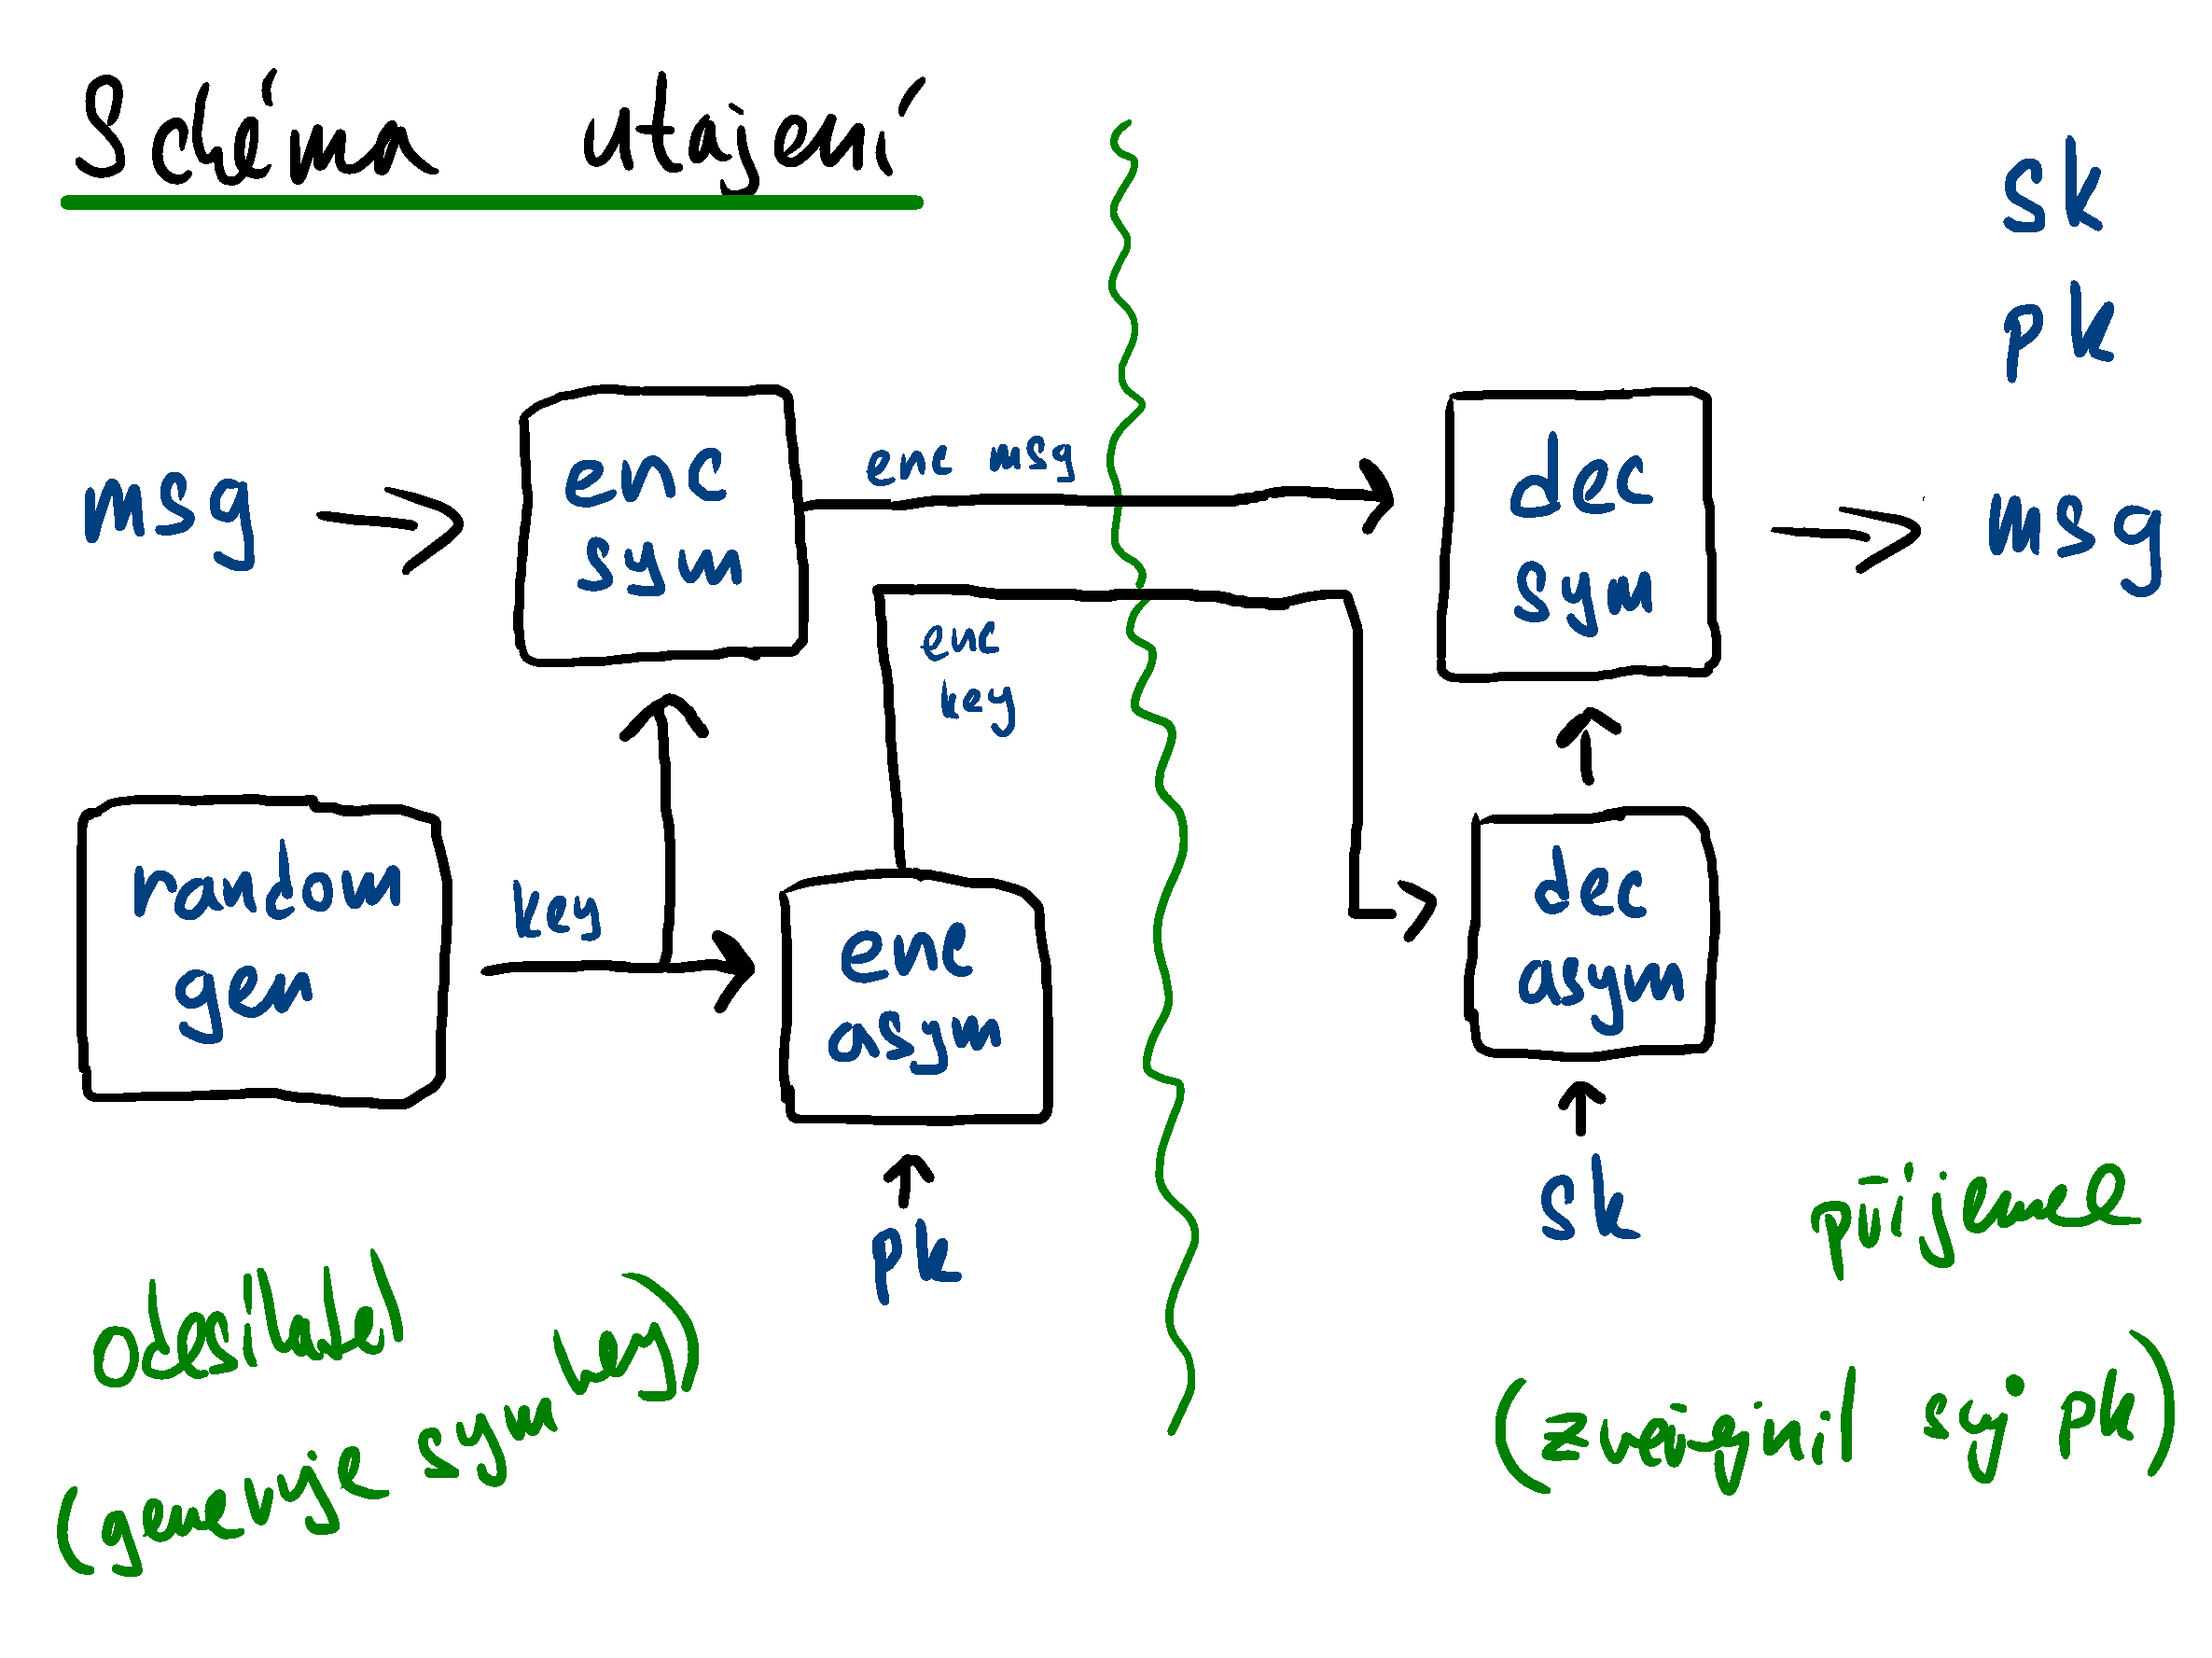
\includegraphics[width=1\linewidth]{kry_2/hybrid_utajeni.pdf}
    \caption{Schéma utajení hybridní kryptografie.}
\end{figure}

\begin{figure}[H]
    \centering
    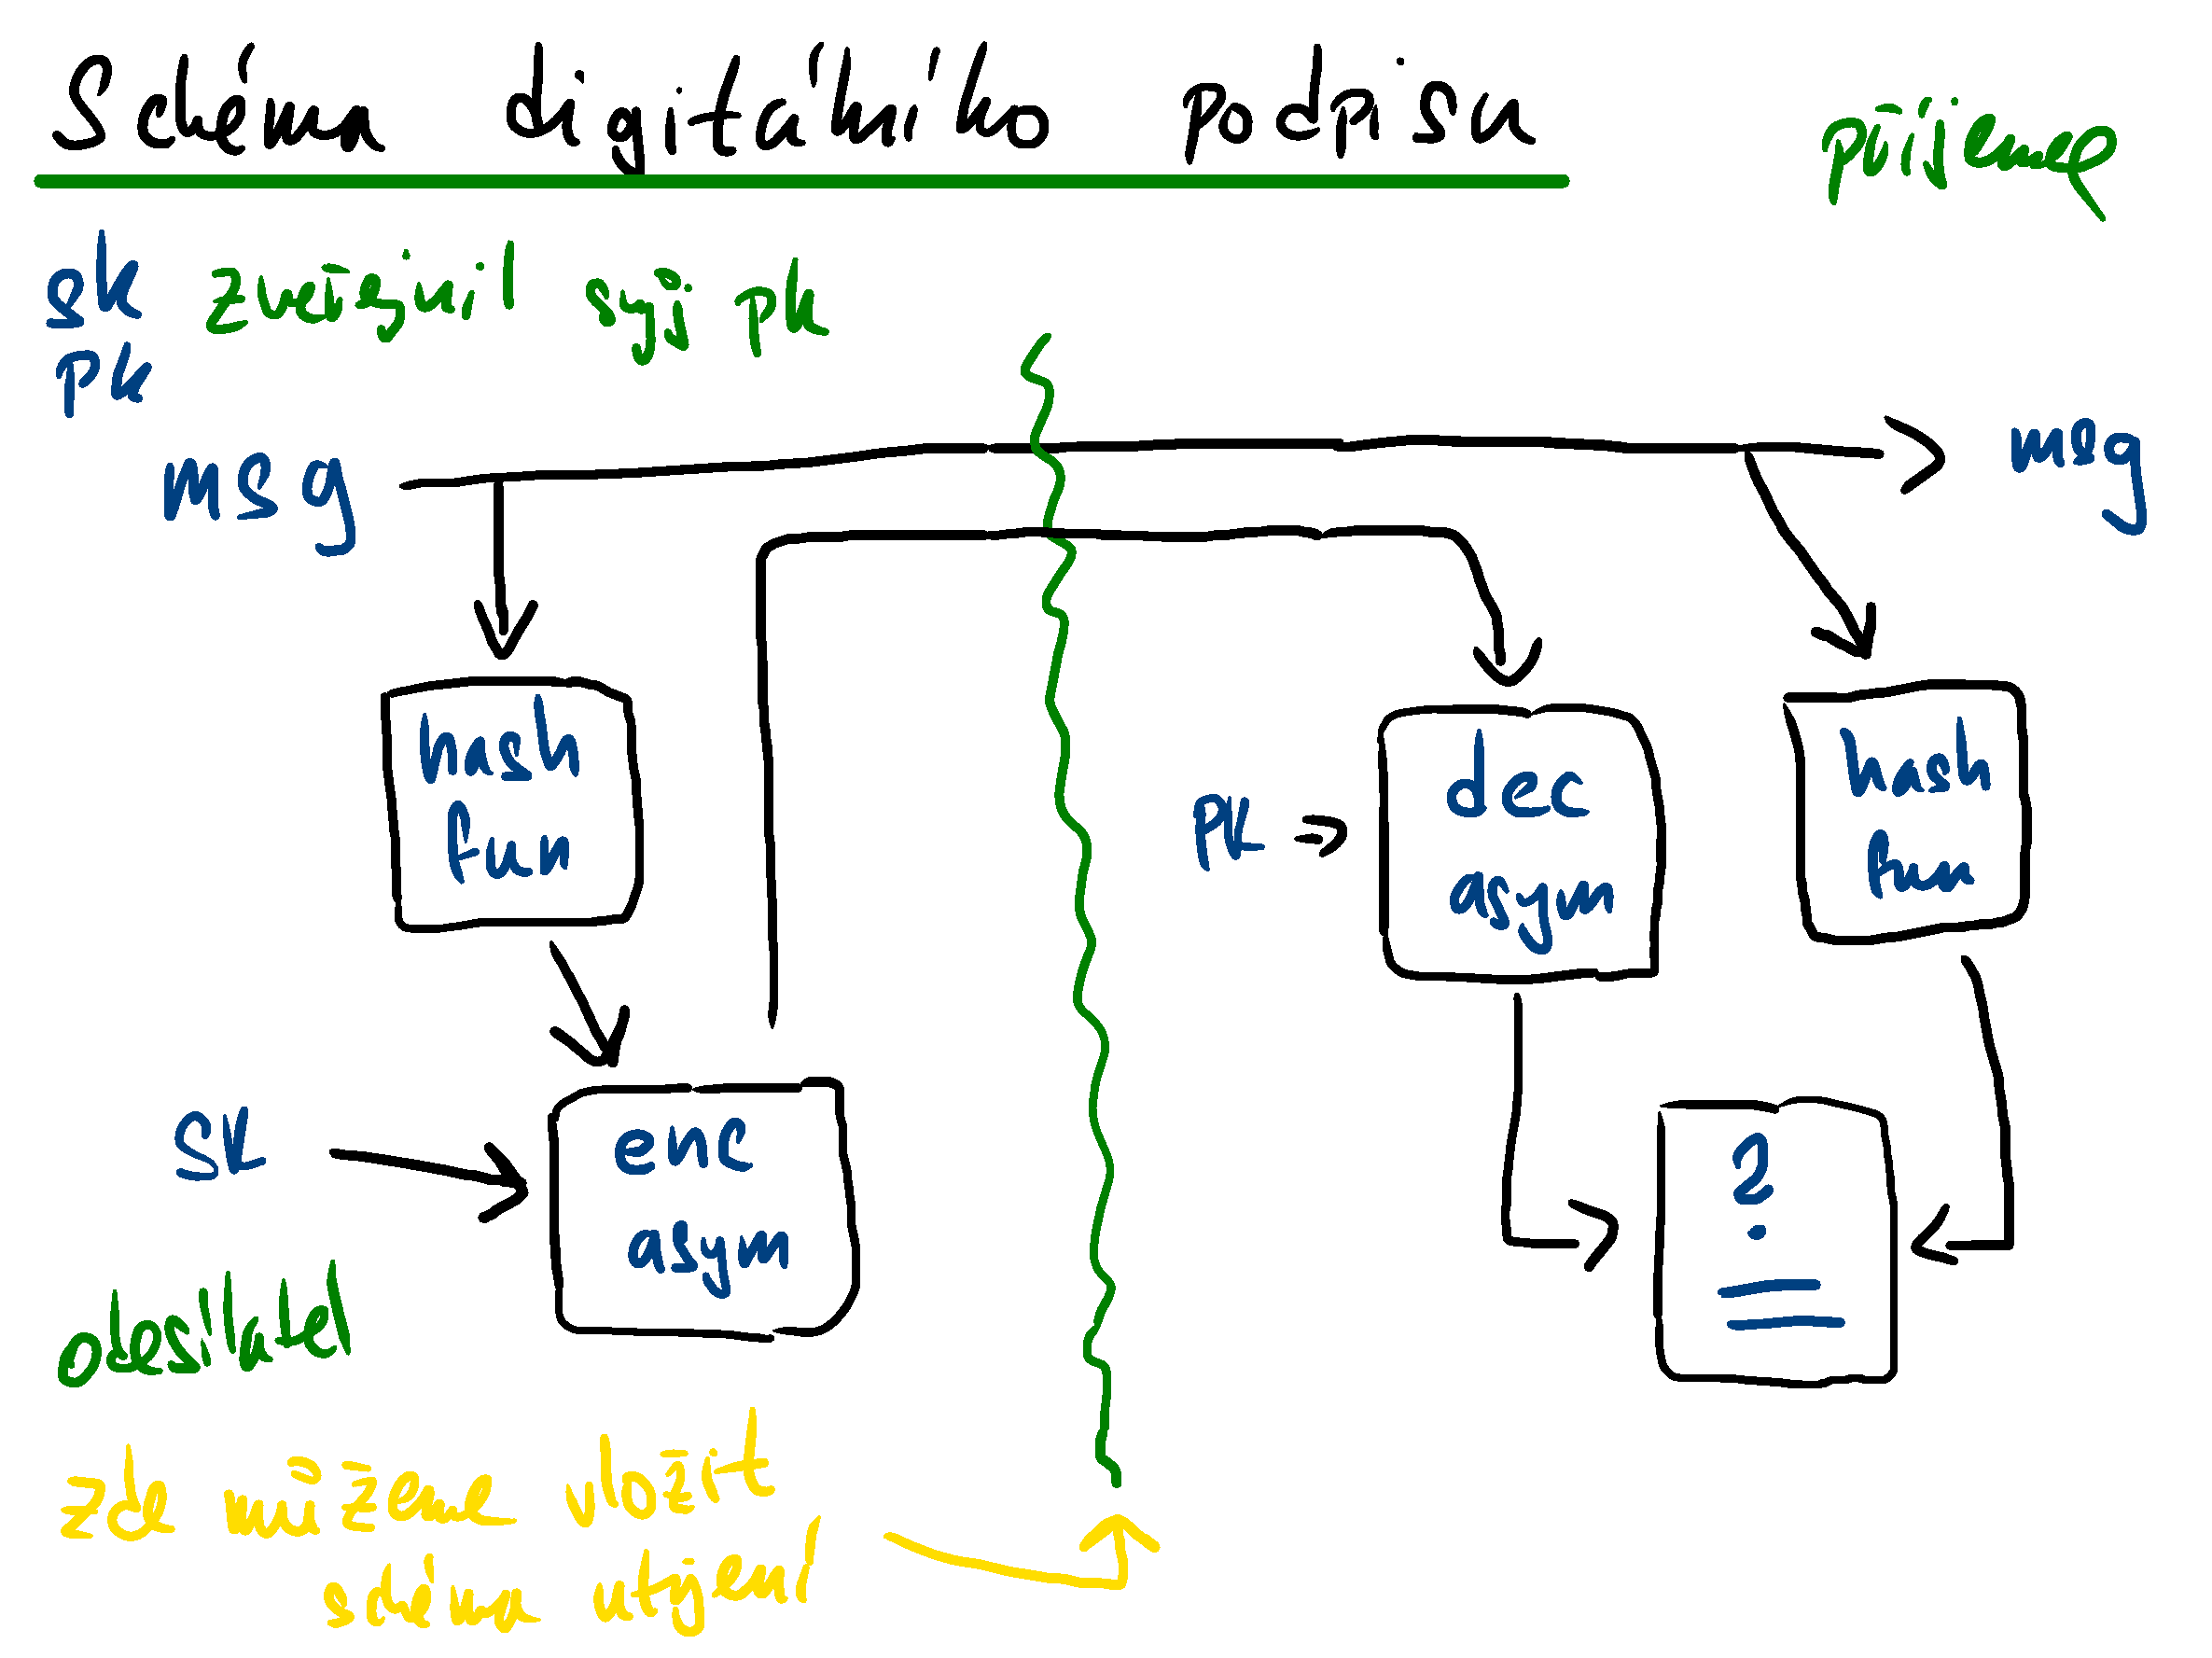
\includegraphics[width=1\linewidth]{kry_2/hybrid_podpis.pdf}
    \caption{Schéma digitálního podpisu hybridní kryptografie.}
\end{figure}

%%%%%%%%%%%%%%%%%%%%%%%%%%%%%%%%%%%%%%%%%%%%%%%%%%%%%%%%%%%%%%%%%%%%%%%%%%%%%%%%

\section{RSA}

Algoritmus RSA (Rivest-Shamir-Adleman) lze použít jak pro šifrování dat pro digitální podepisování. Je založen na problému faktorizace velkých čísel.

\paragraph*{Klíče} Klíče se skládají z: \begin{compactitem}
    \item $p, q$ -- dvě náhodná soukromá prvočísla,
    \item $n$ -- veřejný modul ($n = p \cdot q$),
    \item $e$ -- veřejný exponent ($e < \Phi(n) \; \land \; GCD(\Phi(n), e) = 1$), typicky $3$ nebo $2^{16}+1$\footnote{$GCD$~--~největší společný dělitel},
    \item $d$ -- soukromý exponent,
    \item musí platit vztah: $e \cdot d \; \text{mod} \; \Phi(n) = 1$.
\end{compactitem}

\noindent Veřejný klíč $PK = (n, e)$, soukromý klíč $SK = (n, d)$.

\paragraph*{Postup generování} Postup generování klíčů: \begin{compactenum}
    \item vygenerovat prvočísla $p$ a $q$,
    \item spočítat modul $n = p \cdot q$,
    \item spočítat $\Phi(n) = (p-1) \cdot (q-1)$,
    \item zvolit veřejný exponent $e < \Phi(n) \; \land \;GCD(\Phi(n), e) = 1$,
    \item spočítat soukromý exponent $d$ tak, že platí $e \cdot d \; \text{mod} \; \Phi(n) = 1$.
\end{compactenum}

\paragraph*{Šifrování a dešifrování} Mějme zprávu $m$ reprezentovanou jako celé číslo a zašifrovanou zprávu $c$ reprezentovanou také jako celé číslo. Digitální podpis se vytváří stejným způsobem, pouze se prohodí exponenty.

\begin{equation}
    c = m^e \; \text{mod} \; n
\end{equation}

\begin{equation}
    m = c^d \; \text{mod} \; n
\end{equation}

\paragraph*{Útoky a slabiny} Pokud útočník rozloží číslo $n$ na činitele $p$ a $q$, tak může dopočítat soukromý klíč. Pokud útočník uhádně hodnotu $(p-1) \cdot (q-1)$, tak může dopočítat soukromý klíč. Šifrování malých čísel je zranitelné, proto se používá \uv{předzpracování}~--~zarovnání na $X$ bitů (2048).

\begin{figure}[H]
    \centering
    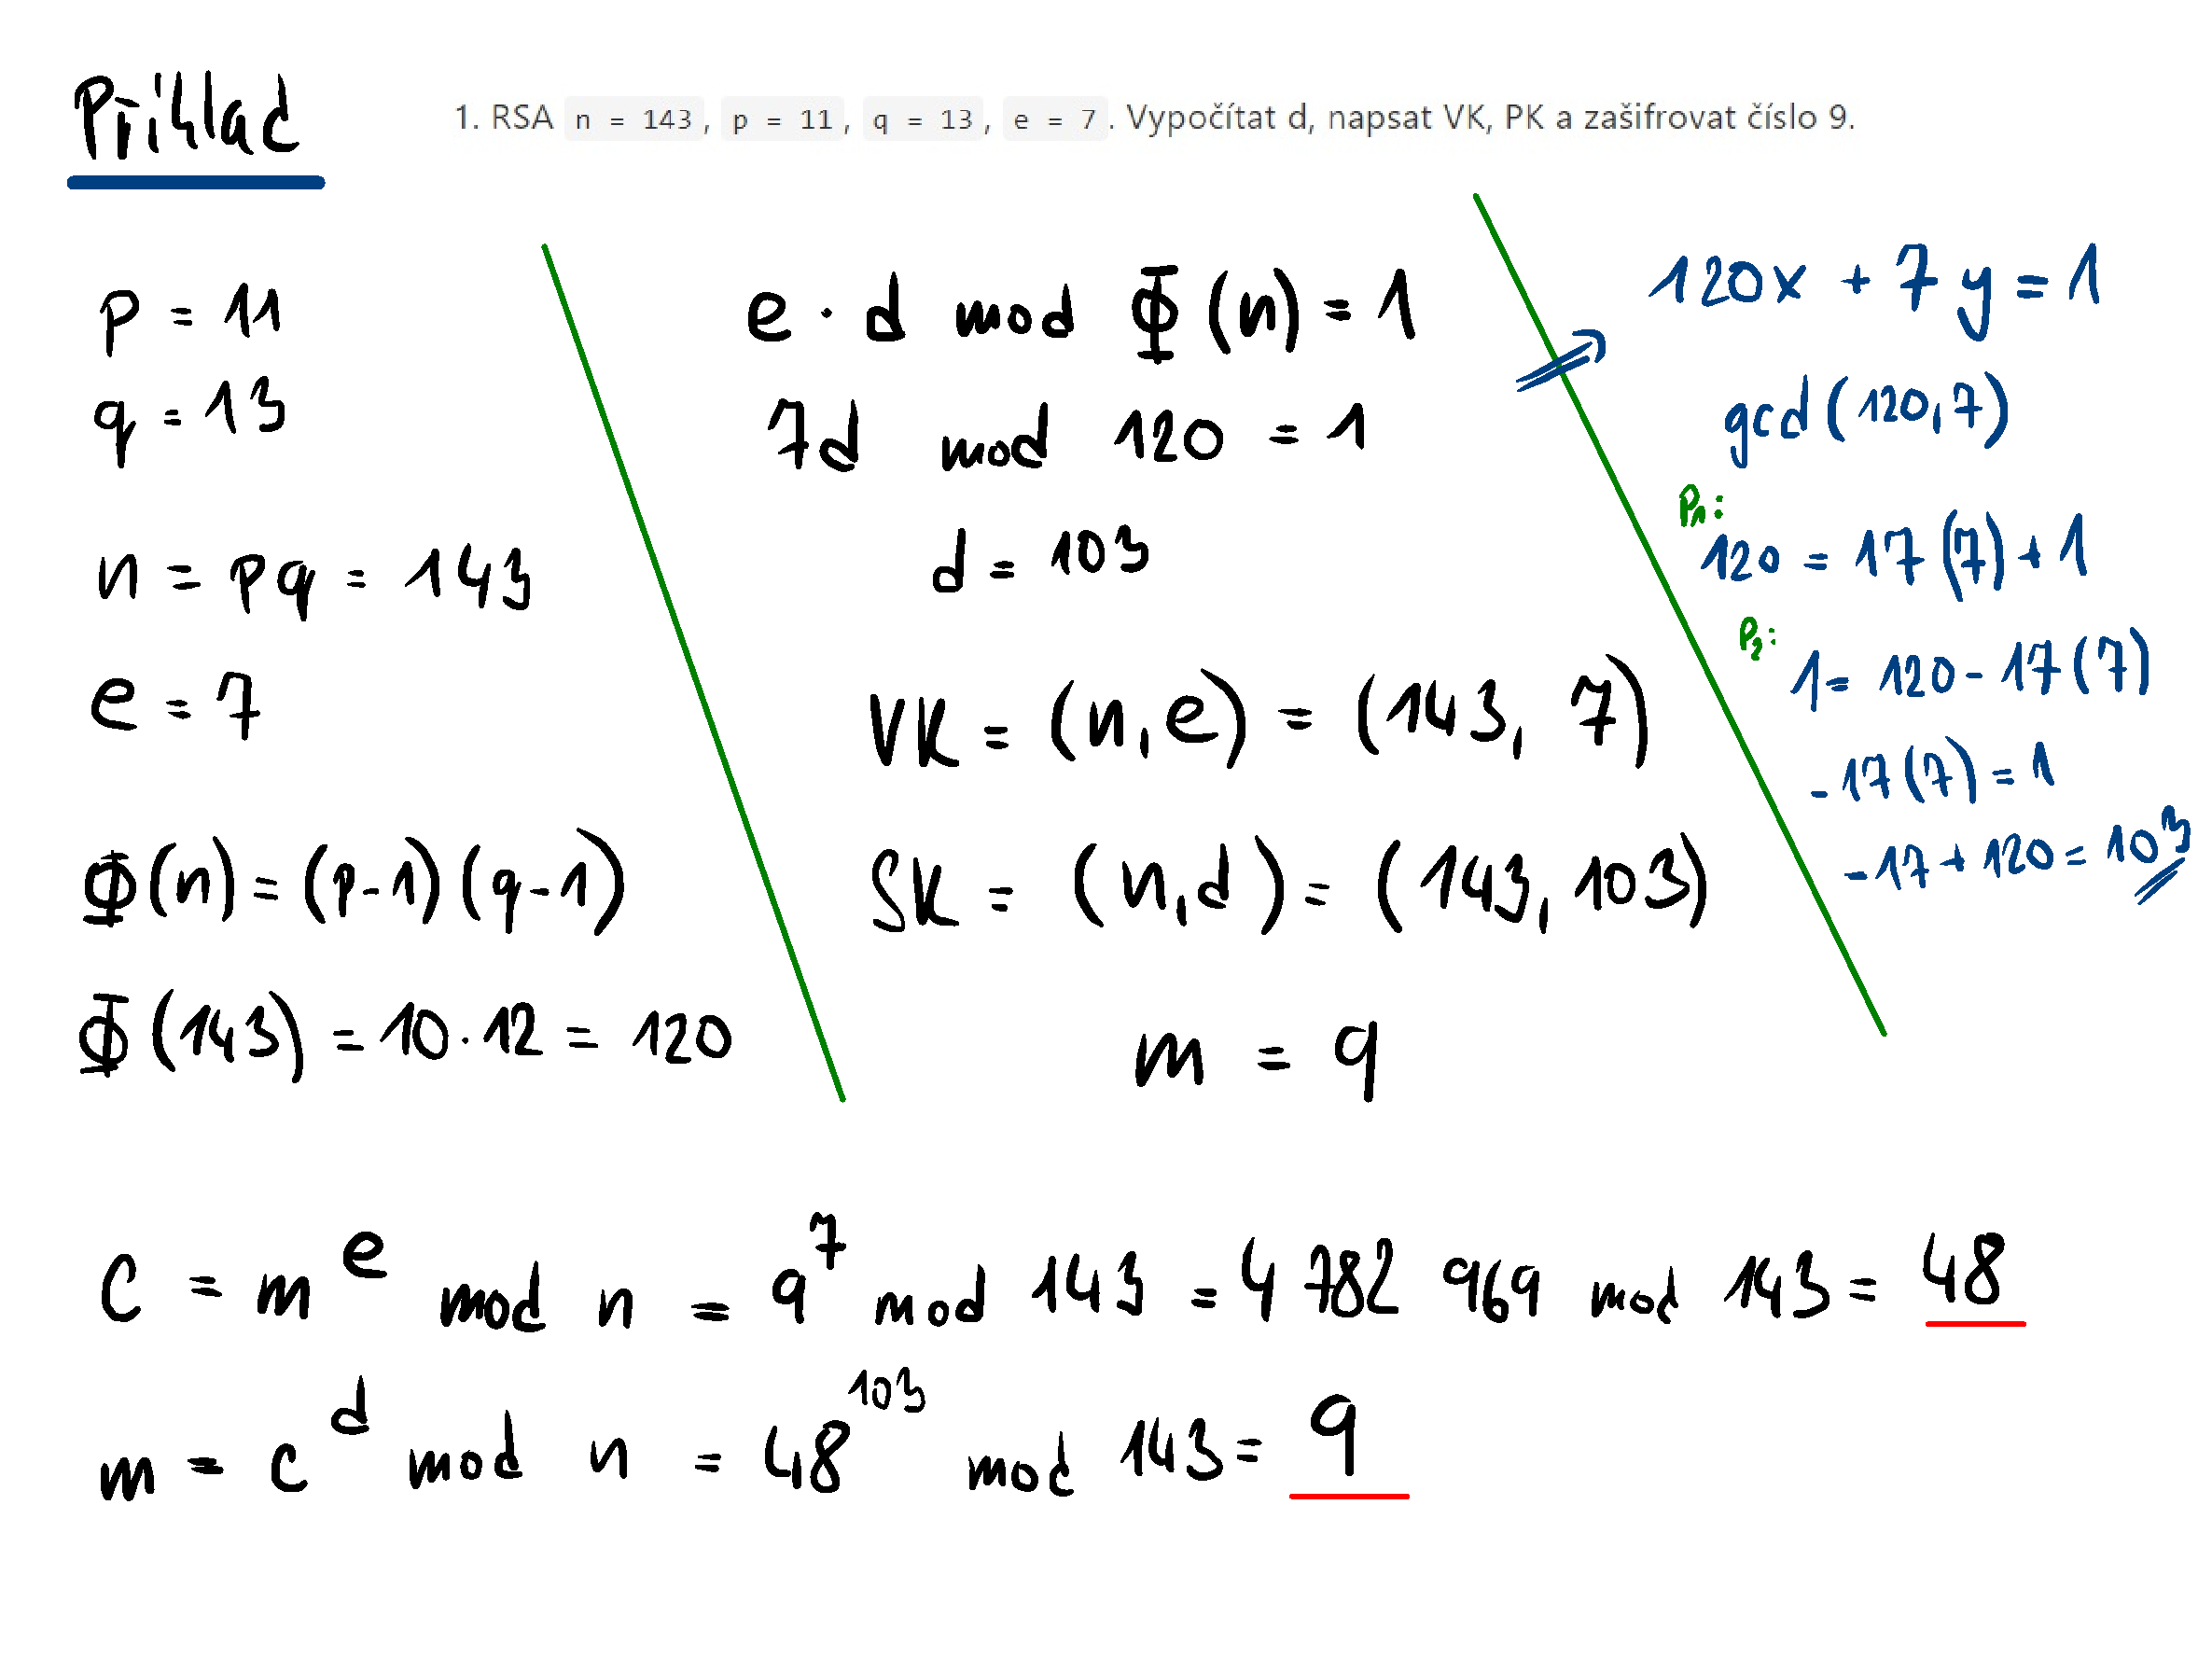
\includegraphics[width=1\linewidth]{kry_2/rsa_example.pdf}
    \caption{Příklad RSA.}
\end{figure}
